\newgeometry{hmargin = 2cm, vmargin = 2cm}
\begin{landscape}
	\section{LTI-Grundglieder \formelbuch{115 \& 201}}
	\usetikzlibrary{arrows}
	\usetikzlibrary{positioning}
	\usetikzlibrary{intersections}
	\usetikzlibrary{decorations.markings}
	\usetikzlibrary{decorations.pathreplacing}
	\tikzset{
		font = \small,
		axis/.style = {
			thick, ->
		},
		line/.style = {
			ultra thick, hsr-blue,
		},
		locus/.style = {
			line,
			postaction = {
				decorate, decoration = {
					markings,
					mark = between positions .2 and .92 step 6mm  with {%
						\draw[ultra thick, ->] (0,0) -- ++(1pt,0);
					},
				},
			},
		},
		dot/.style = {
			circle, draw = hsr-blue, thick,
			fill = white,
			inner sep = 0pt,
			minimum size = 1mm,
		},
		indbrace/.style = {
			gray,
			thick,
			decorate,
			decoration = {
				brace,
				raise = 3pt,
			},
		},
	}
	\centering
	\begin{tabularx}{\linewidth}{%
			% columns with tikz graphics must be of type m{} to get a correct
			% vertical centering
			c % name
			>{\centering}m{4cm} % symbol
			*{2}{ >{\(\displaystyle}X<{\)} } % math stuff
			m{3.5cm} % nyquist
			m{6.5cm} % bode
	}
		\toprule[2pt]

		\bfseries Typ &
		\bfseries Symbol &
		\textbf{Differentialgleichung} &
		\textbf{Frequenzgang } G &
		\bfseries Nyquistdiagramm &
		\bfseries Bodediagramm \\

		\midrule[1pt]\endhead

		%
		% Proportional
		%
		P
		&
		% symbol
		\begin{tikzpicture}
			\node[rtprop] (G) {};
			\node[anchor = south west] at (G.north west) {\(K\)};
			\draw[ultra thick, ->] (G.west) ++(-.5,0) node[left] {\(u\)} -- (G.west);
			\draw[ultra thick, ->] (G.east) -- ++(.5,0) node[right] {\(y\)};
		\end{tikzpicture}
		&
		% diff eq
		y = Ku & K
		&
		% nyquist diagram
		\begin{tikzpicture}
			\draw[axis] (-.2,0) -- (1.8,0) node[right] {Re};
			\draw[axis] (0,-.2) -- (0,.8) node[above] {Im};
			\coordinate (P) at (1.5,0);
			\draw[indbrace] (0,0) -- node[midway, above = 7pt] {\(K\)} (P);
			\node[dot] at (P) {};
		\end{tikzpicture}
		&
		% bode diagram
		\begin{tikzpicture}
			% amplitude
			\draw[axis] (-.2,0) node[left] {0} -- (1.8,0) node[right] {\(\log \omega\)};
			\draw[axis] (0,-.2) -- (0,.8) node[above] {\(|G|_\text{dB}\)};
			\draw[line] (0,.5) -- (1.7,.5);
			\draw[gray, thick, <->] (1,0) -- node[midway, left] {\(K_\text{dB}\)} (1,.5);
			% phase
			\begin{scope}[xshift = 3.5cm]
				\draw[axis] (-.2,0) node[left] {0} -- (1.8,0) node[right] {\(\log \omega\)};
				\draw[axis] (0,-.2) -- (0,.8) node[above] {\(\angle G\)};
				\draw[line] (0,0) -- (1.7,0);
			\end{scope}
		\end{tikzpicture}
		\\

		\midrule[1pt]

		%
		% Delay
		%
		T
		&
		% symbol
		\begin{tikzpicture}
			\node[rtdelay] (G) {};
			\node[anchor = south east] at (G.north east) {\(T_t\)};
			\draw[ultra thick, ->] (G.west) ++(-.5,0) node[left] {\(u\)} -- (G.west);
			\draw[ultra thick, ->] (G.east) -- ++(.5,0) node[right] {\(y\)};
		\end{tikzpicture}
		&
		% diff eq
		y(t) = \varepsilon(t) u(t - T_t) & e^{-j\omega T_t}
		&
		% nyquist diagram
		\begin{tikzpicture}
			\draw[axis] (-1,0) -- (1,0) node[right] {Re};
			\draw[axis] (0,-1) -- (0,1) node[above] {Im};
			\draw[locus] (.75,0) arc (360:0:.75);
			\node[dot] at (.75,0) {};
			\node[below right = .5mm] at (.75,0) {\(\omega = 2\pi n\)};
		\end{tikzpicture}
		&
		% bode diagram
		\begin{tikzpicture}
			% amplitude
			\draw[axis] (-.2,0) node[left] {0} -- (1.8,0) node[right] {\(\log \omega\)};
			\draw[axis] (0,-.8) -- (0,.8) node[above] {\(|G|_\text{dB}\)};
			\draw[line] (0,0) -- (1.7,0);

			% phase
			\begin{scope}[xshift = 3.5cm]
				\draw[axis] (0,-.8) -- (0,.8) node[above] {\(\angle G\)};
				\draw[axis] (-.2,.6) node[left] {0} -- (1.8,.6) node[right] {\(\log \omega\)};
				%% TODO: fix this ugly thing
				\begin{scope}[shift = {(2,.6)}]
					\draw[line, domain = 0.001:1, samples = 60, smooth, variable = \x]
						plot ({log10(\x) / 1.5}, {-\x});
				\end{scope}
			\end{scope}
		\end{tikzpicture}
		\\

		\midrule[1pt]

		%
		% PT1
		%
		PT\(_1\)
		&
		% symbol
		\begin{tikzpicture}
			\node[rtpt1] (G) {};
			\node[anchor = south west] at (G.north west) {\(K\)};
			\node[anchor = south east] at (G.north east) {\(T\)};
			\draw[ultra thick, ->] (G.west) ++(-.5,0) node[left] {\(u\)} -- (G.west);
			\draw[ultra thick, ->] (G.east) -- ++(.5,0) node[right] {\(y\)};
		\end{tikzpicture}
		&
		% diff eq
		T\dot{y} + y = Ku & \frac{K}{j\omega T + 1}
		&
		% nyquist diagram
		\begin{tikzpicture}
			\draw[axis] (-.2,0) -- (1.8,0) node[right] {Re};
			\draw[axis] (0,-1) -- (0,.6) node[above] {Im};
			\draw[locus] (1.5,0) arc (360:180:.75);
			\draw[indbrace] (0,0) -- node[midway, above = 7pt] {\(K\)} (1.5,0);
			\draw
				(0,0) node[dot] {} % node[above left, anchor = south east] {\(\omega\to\infty\)}
				(1.5,0) node[dot] {} node[above right = 2pt, anchor = south west] {\(\omega = 0\)} 
				(.75,-.75) node[dot] {} node[below] {\(\omega = 1/T\)}
			;
		\end{tikzpicture}
		&
		% bode diagram
		\begin{tikzpicture}
			% amplitude
			\draw[axis] (-.2,0) node[left] {0} -- (1.8,0) node[right] {\(\log \omega\)};
			\draw[axis] (0,-.8) -- (0,.8) node[above] {\(|G|_\text{dB}\)};

			\draw[line]
				(0,.5) -- (1,.5)
					node[dot] {}
					node[above, black] {\(\omega = \frac{1}{T}\)}
					--
					node[pos = .9, black, left, anchor = east] {\(-20\frac{\text{dB}}{\text{Dek}}\)}
				(1.7,-.5);
			\draw[gray, thick, <->] (.8,0) -- node[midway, left] {\(K_\text{dB}\)} (.8,.5);

			% phase
			\begin{scope}[xshift = 3.5cm]
				\coordinate (O) at (0,.6);

				\draw[axis] (O)
					++ (-.2,0) node[left] {0} 
					-- ++(2,0) node[right] {\(\log \omega\)};
				\draw[axis] (0,-.8) -- (0,.8) node[above] {\(\angle G\)};

				\draw[line] (0,.6)
					-- (.3,.6) node[dot] {} node[above right, black] {\(\omega = \frac{1}{10 T}\)}
					-- (.8,0) node[dot] (A) {} node[right, black] {\(\omega = \frac{1}{T}\)}
					-- (1.3,-.6) node[dot] (B) {} node[below right, black] {\(\omega = \frac{10}{T}\)}
					-- (1.7,-.6);

				\draw[gray, dashed] (A) -- (O |- A) node[left, black] {\(-\frac{\pi}{4}\)};
				\draw[gray, dashed] (B) -- (O |- B) node[left, black] {\(-\frac{\pi}{2}\)};
			\end{scope}
		\end{tikzpicture}
		\\

		\midrule[1pt]

		%
		% PT2
		%
		PT\(_2\)
		&
		% symbol
		\begin{tikzpicture}
			\node[rtpt2] (G) {};
			\node[anchor = south west] at (G.north west) {\(K\)};
			\node[anchor = south] at (G.north) {\(\zeta\)};
			\node[anchor = south east] at (G.north east) {\(T\)};
			\draw[ultra thick, ->] (G.west) ++(-.5,0) node[left] {\(u\)} -- (G.west);
			\draw[ultra thick, ->] (G.east) -- ++(.5,0) node[right] {\(y\)};
		\end{tikzpicture}
		&
		% diff eq
		T^2 \ddot{y} + 2\zeta T \dot{y} + y = Ku &
		\frac{K}{T^2 (j\omega)^2 + 2\zeta T (j\omega) + 1} 
		&
		% nyquist diagram
		\begin{tikzpicture}
			\draw[axis] (-.2,0) -- (1.8,0) node[right] {Re};
			\draw[axis] (0,-1) -- (0,.6) node[above] {Im};

			\draw[locus] (1.5,0) 
				to[out = -90, in = 0] (.75,-.8)
				to[out = 180, in = -30] (0, -.7)
				to[out = 160, in = 190] (0,0)
			;

			\draw[indbrace] (0,0) -- node[midway, above = 7pt] {\(K\)} (1.5,0);
			\draw
				(0,0) node[dot] {} % node[above left, anchor = south east] {\(\omega\to\infty\)}
				(1.5,0) node[dot] {} node[above right = 2pt, anchor = south west] {\(\omega = 0\)} 
				(0,-.7) node[dot] {} node[below left = 4pt, anchor = north west] {\(\omega = 1/T\)}
			;
		\end{tikzpicture}
		&
		% bode diagram
		\begin{tikzpicture}
			% amplitude
			\draw[axis] (-.2,0) node[left] {0} -- (1.8,0) node[right] {\(\log \omega\)};
			\draw[axis] (0,-.8) -- (0,.8) node[above] {\(|G|_\text{dB}\)};

			\draw[line] (0,.5)
				-- (.8,.5)  node[dot] (A) {}
				-- (1,.7)   node[dot] (B) {} node[above, black] {\(\omega = \frac{1}{T}\)} % node[black, right] {\(\sim Q\)}
				-- (1.2,.22) node[dot] (C) {}
				-- node[pos = .9, black, left, anchor = east] {\(-40\frac{\text{dB}}{\text{Dek}}\)}
				(1.7,-.5);

			\draw[gray, thick] (A) -- (1,.5) -- (C);
			\draw[gray, thick, <->] (.2,0) -- node[midway, right] {\(K_\text{dB}\)} (.2,.5);

			% phase
			\begin{scope}[xshift = 3.5cm]
				\coordinate (O) at (0,.6);

				\draw[axis] (O)
					++ (-.2,0) node[left] {0} 
					-- ++(2,0) node[right] {\(\log \omega\)};
				\draw[axis] (0,-.8) -- (0,.8) node[above] {\(\angle G\)};

				\draw[line] (0,.6)
					-- (.3,.6) node[dot] {} node[above right, black] {\(\omega = \frac{1}{10 T}\)}
					-- (.8,0) node[dot] (A) {} node[right, black] {\(\omega = \frac{1}{T}\)}
					-- (1.3,-.6) node[dot] (B) {} node[below right, black] {\(\omega = \frac{10}{T}\)}
					-- (1.7,-.6);

				\draw[gray, dashed] (A) -- (O |- A) node[left, black] {\(-\frac{\pi}{2}\)};
				\draw[gray, dashed] (B) -- (O |- B) node[left, black] {\(-\pi\)};
			\end{scope}
		\end{tikzpicture}
		\\

		\midrule[1pt]

		%
		% Integrator
		%
		I
		&
		% symbol
		\begin{tikzpicture}
			\node[rtint] (G) {};
			\node[anchor = south west] at (G.north west) {\(K\)};
			\draw[ultra thick, ->] (G.west) ++(-.5,0) node[left] {\(u\)} -- (G.west);
			\draw[ultra thick, ->] (G.east) -- ++(.5,0) node[right] {\(y\)};
		\end{tikzpicture}
		&
		% diff eq
		\dot{y} = K u & \frac{K}{j\omega}
		&
		% nyquist diagram
		\begin{tikzpicture}
			\draw[axis] (-.2,0) -- (1.8,0) node[right] {Re};
			\draw[axis] (0,-1) -- (0,.3) node[above] {Im};

			\draw[locus] (0,-1) -- (0,0);
			\draw
				(0,0) node[dot] {} node[above right = 2pt] {\(\omega\to\infty\)}
				(0,-.5) node[dot] {} node[left] {\(j\)}
			;
		\end{tikzpicture}
		&
		% bode diagram
		\begin{tikzpicture}
			% amplitude
			\begin{scope}[yshift = 2.5mm]
				\draw[axis] (0,0)
					++ (-.2,0) node[left] {0}
					-- ++(2,0) node[right] {\(\log \omega\)};

				\draw[axis] (0,0)
					++(0,-.5) 
					-- ++(0,1) node[above] {\(|G|_\text{dB}\)};

				\draw[line] (0,.3)
					-- (.8,0) node[dot] {} node[black, above right] {\(\omega = \frac{1}{K}\)}
					-- (1.6,-.3);
			\end{scope}

			% phase
			\begin{scope}[xshift = 3.5cm]
				\coordinate (O) at (0,.6);
				\draw[axis] (O)
					++ (-.2,0) node[left] {0} 
					-- ++(2,0) node[right] {\(\log \omega\)};

				\draw[axis] (0,-.2) -- (0,.8) node[above] {\(\angle G\)};
				\draw[line] (0,0) node[left, black] {\(-\frac{\pi}{2}\)} -- (1.7,0);
			\end{scope}
		\end{tikzpicture}
		\\

		\midrule[1pt]

		%
		% Proportional with Integrator
		%
		PI
		&
		% symbol
		\begin{tikzpicture}
			\node[rtpi] (G) {};
			\node[anchor = south west] at (G.north west) {\(K\)};
			\node[anchor = south east] at (G.north east) {\(T\)};
			\draw[ultra thick, ->] (G.west) ++(-.5,0) node[left] {\(u\)} -- (G.west);
			\draw[ultra thick, ->] (G.east) -- ++(.5,0) node[right] {\(y\)};
		\end{tikzpicture}
		&
		% diff eq
		y = K_R \left( u + \int_0^t \frac{u ~d\tau}{T} \right) &
		K \left( 1 + \frac{1}{j\omega T} \right)
		&
		% nyquist diagram
		\begin{tikzpicture}
			\draw[axis] (-.2,0) -- (1.8,0) node[right] {Re};
			\draw[axis] (0,-1) -- (0,.4) node[above] {Im};

			\draw[locus] (.7,-1) -- (.7,0);
			\draw[indbrace] (0,0) -- node[midway, above = 7pt] {\(K\)} (.7,0);
			\draw
				(.7,0) node[dot] {} node[above right = 2pt] {\(\omega\to\infty\)}
			;
		\end{tikzpicture}
		&
		% bode diagram
		%% TODO: complete missing bode diagram for PI
		\\

		\midrule[1pt]

		%
		% Differentiator
		%
		D
		&
		% symbol
		\begin{tikzpicture}
			\node[rtdiff] (G) {};
			\node[anchor = south west] at (G.north west) {\(K\)};
			\draw[ultra thick, ->] (G.west) ++(-.5,0) node[left] {\(u\)} -- (G.west);
			\draw[ultra thick, ->] (G.east) -- ++(.5,0) node[right] {\(y\)};
		\end{tikzpicture}
		Nicht realisierbar!
		&
		% diff eq
		y = K\dot{u} & j\omega K
		&
		% nyquist diagram
		\begin{tikzpicture}
			\draw[axis] (-.2,0) -- (1.8,0) node[right] {Re};
			\draw[axis] (0,-.3) -- (0,1) node[above] {Im};

			\draw[locus] (0,0) -- (0,1);
			\draw
				(0,0) node[dot] {} node[below right = 2pt] {\(\omega = 0\)}
			;
		\end{tikzpicture}
		&
		% bode diagram
		\begin{tikzpicture}
			% amplitude
			\begin{scope}[yshift = 2.5mm]
				\draw[axis] (0,0)
					++ (-.2,0) node[left] {0}
					-- ++(2,0) node[right] {\(\log \omega\)};

				\draw[axis] (0,0)
					++(0,-.5) 
					-- ++(0,1) node[above] {\(|G|_\text{dB}\)};

				\draw[line] (0,-.3)
					-- (.8,0) node[dot] {} node[black, below] {\(\omega = \frac{1}{K}\)}
					-- (1.6,.3);
			\end{scope}

			% phase
			\begin{scope}[xshift = 3.5cm]
				\coordinate (O) at (0,0);
				\draw[axis] (O)
					++ (-.2,0) node[left] {0} 
					-- ++(2,0) node[right] {\(\log \omega\)};

				\draw[axis] (0,-.2) -- (0,.8) node[above] {\(\angle G\)};

				\draw[line] (0,.6) node[left, black] {\(\frac{\pi}{2}\)} -- (1.7,.6);
			\end{scope}
		\end{tikzpicture}
		\\

		\midrule[1pt]

		%
		% Real differentiator
		%
		DT\(_1\)
		&
		% symbol
		\begin{tikzpicture}
			\node[rtdt1] (G) {};
			\node[anchor = south west] at (G.north west) {\(K\)};
			\node[anchor = south east] at (G.north east) {\(T\)};
			\draw[ultra thick, ->] (G.west) ++(-.5,0) node[left] {\(u\)} -- (G.west);
			\draw[ultra thick, ->] (G.east) -- ++(.5,0) node[right] {\(y\)};
		\end{tikzpicture}
		&
		% diff eq
		T\dot{y} + y = K\dot{u} & \frac{j\omega K}{1 + j\omega T}
		&
		% nyquist diagram
		\begin{tikzpicture}
			\draw[axis] (-.2,0) -- (1.8,0) node[right] {Re};
			\draw[axis] (0,-.5) -- (0,1.1) node[above] {Im};
			\draw[locus] (0,0) arc (180:0:.75);
			\draw[indbrace] (1.5,0) -- node[midway, below = 7pt] {\(K\)} (0,0);
			\draw
				(0,0) node[dot] {}
				(1.5,0) node[dot] {} node[below right = 2pt, anchor = north west] {\(\omega\to\infty\)} 
				(.75,.75) node[dot] {} node[above] {\(\omega = 1/T\)}
			;
		\end{tikzpicture}
		&
		% bode diagram
		%% TODO: complete missing bode diagram for DT1
		\\

		\bottomrule[2pt]
	\end{tabularx}

	\begin{multicols*}{2}
		\raggedright
		%% TODO: finish
		% \subsection{\"Aquivalente Glieder}
		% \begin{center}
		% 	\begin{tikzpicture}
		% 		\matrix[column sep = 5mm]{
		% 			\node[rtpi] {}; &
		% 			\node {\(=\)}; &
		% 			\node[rtprop] (P) {};
		% 			\node[rtint, right = 7mm of P] (I) {}; \\
		% 		};
		% 		\draw[ultra thick, ->] (P.west) ++(-.4,0) -- (P.west);
		% 		\draw[ultra thick, ->] (P) -- (I);
		% 		\draw[ultra thick, <-] (I.east) ++(.4,0) -- (I.east);
		% 	\end{tikzpicture}
		% \end{center}

		% \begin{center}
		% 	\begin{tikzpicture}
		% 		\matrix[column sep = 5mm]{
		% 			\node[rtpt1] {}; &
		% 			\node {\(=\)}; \\
		% 		};
		% 	\end{tikzpicture}
		% \end{center}

		\subsection{Schaltungen}
		\begin{figure}[H]
			\centering
			\begin{tikzpicture}[
					node distance = 1mm,
					wire/.style = {ultra thick}
				]
				% series
				\begin{scope}
					\matrix (M) [column sep = 7mm, nodes = {rtbox}]{
						\node (G1) {\(G_1\)}; & \node (G2) {\(G_2\)}; \\
					};
					
					\node[above = 8mm of M] {Serieschaltung \(G = G_1 \cdot G_2\)};

					\draw[wire, ->] (G1.west) ++(-.5,0) node[left] {\(u\)} -- (G1.west);
					\draw[wire, ->] (G1) -- (G2);
					\draw[wire, <-] (G2.east) ++(.5,0) node[right] {\(y\)} -- (G2.east);
				\end{scope}

				% parallel
				\begin{scope}[xshift = 6cm]
					\matrix (M) [row sep = 1mm, column sep = 7mm, nodes = {rtbox}]{
						& \node[rtbox] (G1) {\(G_1\)}; \\
						\node[rtsplit] (L) {}; & & \node[rtsum] (R) {}; \\
						& \node[rtbox] (G2) {\(G_2\)}; \\
					};
					
					\node[above = of M] {Parallelschaltung \(G = G_1 + G_2\)};

					\draw[wire] (L.west) ++(-.5,0) node[left] {\(u\)} -- (L.west);
					\draw[wire, ->] (L) |- (G1);
					\draw[wire, ->] (L) |- (G2);
					\draw[wire, ->] (G1) -| node[pos = .9, right] {\(+\)} (R);
					\draw[wire, ->] (G2) -| node[pos = .9, right] {\(+\)} (R);
					\draw[wire, <-] (R.east) ++(.5,0) node[right] {\(y\)} -- (R.east);
				\end{scope}

				% negative feedback
				\begin{scope}[yshift = -4cm]
					\matrix (M) [row sep = 4mm, column sep = 7mm] {
						\node[rtsum] (L) {}; & \node[rtbox] (G0) {\(G_0\)}; & \node[rtsplit] (R) {}; \\
						& \node[rtbox] (GF) {\(G_F\)}; \\
					};

					\node[above = of M] {R\"uckkopplung \(\displaystyle G = \frac{G_0}{1 + G_0 \cdot G_F}\)};

					\draw[wire, ->] (L.west) ++(-.5,0) node[left] {\(u\)} -- node[pos = .6, below] {\(+\)} (L.west);
					\draw[wire, ->] (L) -- (G0);
					\draw[wire] (G0) -- (R);
					\draw[wire, ->] (R) |- (GF);
					\draw[wire, ->] (GF) -| node[pos = .9, left] {\(-\)} (L);
					\draw[wire, <-] (R.east) ++(.5,0) node[right] {\(y\)} -- (R.east);
				\end{scope}

				% mason's rule
				\begin{scope}[yshift = -4cm, xshift = 6cm]
					%% TODO: mason's rule
				\end{scope}
			\end{tikzpicture}
		\end{figure}

		\subsection{PT\(_2\)--Glied}

		\subsubsection{D\"ampfung}
		\[
			K/G_{\text{PT}_2} = T^2 (j\omega)^2 + 2 \zeta T (j\omega) + 1
			= \begin{cases}
				\text{aperiodisch} & \zeta = 1     \\
				\text{stabil}      & 0 < \zeta < 1 \\
				\text{grenzstabil} & \zeta = 0     \\
				\text{instabil}    & \zeta < 0 
			\end{cases}
		\]

		\subsubsection{Sprungantwort}
		\begin{figure}[H]
			\centering
			\begin{tikzpicture}[
				dot/.style = {
					circle, draw = hsr-blue, thick,
					fill = white,
					inner sep = 0pt,
					minimum size = 1mm,
				},
				% PT2 step response
				declare function  = {
					pt2step(\t, \Kv, \Tv, \zetav) = 
						\scale * \Kv * (
							1 - exp(-\zetav * \t / \Tv) * (
								cos(sqrt(1 - \zetav * \zetav) * \t / \Tv * 180 / pi)
								+ \zetav / sqrt(1 - \zetav * \zetav) * sin(sqrt(1 - \zetav * \zetav) * \t / \Tv * 180 / pi)
							)
						);
				},
			]
				% parameters
				\pgfmathsetmacro{\Kv}{2}
				\pgfmathsetmacro{\Tv}{.4}
				\pgfmathsetlengthmacro{\zetav}{.15}

				% help macros
				\pgfmathsetlengthmacro{\scale}{.8 * \linewidth / 10}

				\pgfmathsetlengthmacro{\omegav}{1 / \Tv}
				\pgfmathsetlengthmacro{\omegan}{\omegav * sqrt(1 - \zetav * \zetav)}

				\pgfmathsetlengthmacro{\Ta}{(pi - acos(\zetav) * pi / 180) / \omegan}
				\pgfmathsetlengthmacro{\Tm}{pi / \omegan}
				\pgfmathsetlengthmacro{\Tn}{2 * pi / \omegan}

				\coordinate (O) at (0,0);

				% axis
				\draw[thick, <->] (.8 * \linewidth,0) node[right] {\(t\)} 
					-- (0,0) -- (0,{2 + \Kv}) node[above] {\(y\)};

				% plots
				\begin{scope}[xshift = 1cm]
					%% step
					\draw[very thick, hsr-mauve, text = black] (0,0) 
						node[below] {\(0\)} -- ++(0,1) -- (9,1);

					%% lower bound 
					\draw[thick, gray, dashed, smooth, samples = 100, variable = \t, domain = 0:9] 
						plot ({\t * \scale}, {
							\scale * \Kv * (1 - exp(-\zetav * \t / \Tv))
						});

					%% stationary value 
					\draw[thick, dashed, hsr-mauve] (0,1) -- (0,\Kv) -- ++(9,0);
					
					%% response
					\draw[very thick, hsr-blue, samples = 180, variable = \t, domain = 0:9]
						plot ({\t * \scale}, {pt2step(\t, \Kv, \Tv, \zetav)});

					% annotations

					\node[dot] (Ta) at ({\Ta * 1cm}, {\Kv}) {};
					\node[dot] (Tm) at ({\Tm * 1cm}, {pt2step({\Tm}, \Kv, \Tv, \zetav)}) {};
					\node[dot] (Tn) at ({\Tn * 1cm}, {pt2step({\Tn}, \Kv, \Tv, \zetav)}) {};
					\node[dot] (Tn2) at ({\Tn * 2 * 1cm}, {pt2step({\Tn * 2}, \Kv, \Tv, \zetav)}) {};
					\node[dot] (Tn3) at ({\Tn * 3 * 1cm}, {pt2step({\Tn * 3}, \Kv, \Tv, \zetav)}) {};

					\draw[draw = gray, text = black, densely dotted]
						% vertical
						(Ta) -- (Ta |- O) node[below] {\(T_a\)}
						(Tm) -- (Tm |- O) node[below] {\(T_m\)}
						(Tn) -- (Tn |- O) node[below] {\(T_n\)}
						(Tn2) -- (Tn2 |- O) node[below] {\(2 T_n\)}
						(Tn3) -- (Tn3 |- O) node[below] {\(3 T_n\)}
						% horizontal
						(Tm) -- (Tm -| O) node[left] {\(y_m\)}
						(0,\Kv) -- ++(-1,0) node[left] {\(y_\infty = K\)}
						(0,1) -- ++(-1,0) node[left] {\(1\)}
					;

					% text
					\node[above, xshift = 3mm, hsr-blue, fill = white] at (Tn2 |- O) {\(\displaystyle
						K \left[ 1 - e^{-\zeta t / T} \left(
							\cos(\omega_n t) +
							\zeta / \sqrt{1 - \zeta^2} \sin(\omega_n t)
						\right)\right]
					\)};

					\node[above = 2mm, xshift = 5mm] at (Tm) {\(
						y_m = y_\infty e^{-\pi\zeta/\sqrt{1-\zeta^2}}
					\)};

					\matrix[fill = white, anchor = south west, column sep = 5mm] at ({1.5 cm * \Tn}, 2.75) {
						\node {\(\omega = 1 / T, \quad \omega_n = 1 / T_n = \omega \sqrt{1 - \zeta^2}\)}; \\
						\node {\(T_a = (\pi - \arccos\zeta) / \omega_n\)}; \\
						\node {\(T_m = T_n / 2 = \pi / \omega_n\)}; \\
					};
				\end{scope}
			\end{tikzpicture}
		\end{figure}
	\end{multicols*}
\end{landscape}
\restoregeometry

\subsubsection{Parameter der Sprungantwort}
\renewcommand{\arraystretch}{1.8}
\begin{tabular}{|m{7cm}|m{1cm}m{0.5cm}m{8cm}}
  \cline{1-1}
  $y_{\infty} =A \cdot K$ & &
  $y_{\infty}$: & Endwert\\
  \cline{1-1}  
	$T_\omega = 2T_m=\dfrac{2\pi}{\omega_n \sqrt{1-\zeta^2}}=\dfrac{2\pi}{\omega}$ & &
	$T_{\omega}$: & Schwingungsdauer \\
  \cline{1-1}
	$\varepsilon = \dfrac{\Delta y}{y_{\infty}}$ & &
	\parbox{0.5cm}{
		$\varepsilon$:\\
		$\Delta y$:
	} & 
	\parbox{8cm}{
		Verhältnis von Überschwinger nach $T_e$ zum Endwert\\
		Toleranzbereich der Amplitude nach $T_e$
	}\\
  \cline{1-1}  
	$T_e = \dfrac{\ln\left(\varepsilon\sqrt{1-\zeta^2}\right)}{-\omega_n\cdot\zeta} = 
	\dfrac{1}{\sigma}\ln\left(\dfrac{\varepsilon\omega}{\omega_n}\right)$ & &
	$T_e$: & Einschwingzeit \\
  \cline{1-1}  
	$T_m = \dfrac{\pi}{\omega_n\sqrt{1-\zeta^2}}=\dfrac{\pi}{\omega}$ & &
	$T_m$: & Überschwingungsdauer\\
  \cline{1-1}  
	$y_m = y_{\infty} \cdot e^{\frac{-\pi\cdot\zeta}{\sqrt{1-\zeta^2}}}$ & &
	$y_m$: & Überschwingweite\\
   \cline{1-1}  
	$\omega = \dfrac{1}{T}\sqrt{1-\zeta^2}= \omega_n\sqrt{1-\zeta^2}=\dfrac{2\pi}{T_\omega}=2\pi f$ & &
	$\omega$: & Kreisfrequenz \\
  \cline{1-1}  
	$\omega_n = \dfrac{1}{T}$ & &
	$\omega_n$: & Kennkreisfrequenz \\
  \cline{1-1}  
	$T_a = \frac{\pi - \arccos{(\zeta)}}{\omega_n\cdot\sqrt{1-\zeta^2}}$ & &
	$T_a$: & Anschwingzeit/Anregelzeit \\
  \cline{1-1}  
	$\sigma = -\dfrac{\zeta}{T} = -\zeta\omega_n$ & &
	$\zeta$: & Dämpfungskonstante \\
  \cline{1-1}
	$\delta = \ln{\Big(\frac{y_i}{y_{i+1}}\Big)} = \frac{2\pi \zeta}{\sqrt{1-\zeta^2}}$ & &
	$\delta$: & Logarithmisches Dekrement\\
  \cline{1-1}  
\end{tabular}
\renewcommand{\arraystretch}{1}
	
\subsubsection{Sprungantwort}
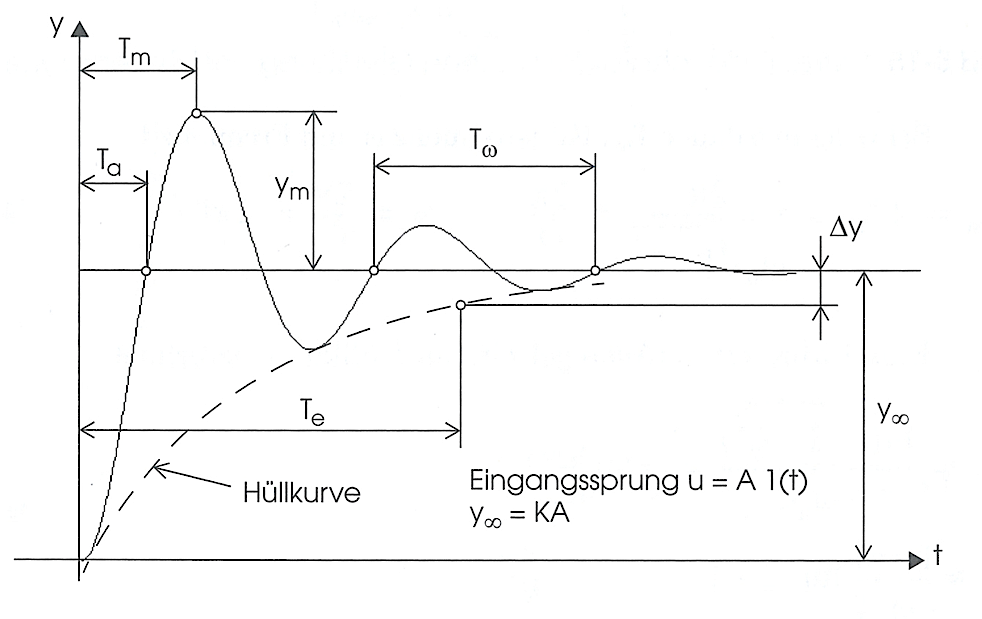
\includegraphics[width = 9cm]{./images/pt2StepResp}

\subsubsection{Dämpfung}
Optimal bei $\zeta=\frac{1}{\sqrt{2}}$ ($\Psi=45$).
Dabei erreicht die Regelgrösse $y$ nach $4.3\%$ Überschwingen rasch den	Endwert.

\subsubsection{Berechnung $\zeta$}
\textbf{Aus DGL} $\ddot{y}+a_1\dot{y}+a_0 y=\ldots$ folgt $a_1=2\zeta\omega_n$, 
$a_0=\omega_n^2$
$\Rightarrow \zeta=\frac{a_1}{2\sqrt{a_0}}$ \\
\textbf{Mittels Überschwingweite} kann $\zeta$ ebenfalls berechnet werden\\
\begin{tabular}{p{2.5cm}p{2.5cm}p{4cm}}
$\zeta = \frac{1}{\sqrt{1+(\frac{\pi}{c})^2}}$ & $c =ln(\frac{y_m}{y_{\infty}})$ & $y_m$: Überschwingweite
\end{tabular}

Weitere Formeln in der LTI-Grundglieder Tabelle
